Database operations are commonly described in the form of relational
algebra, a set of well-defined operations on relations (or tables).
The relational model was designed to enhance human productivity
working with large amounts of data \cite{bratbergsengen}. Relational
algebra makes no assumptions about the underlying algorithms or data
structures, but provide clear definitions of expected behavior.  The
advantage of this separation is that it allows developers to implement
efficient algorithms tailored for different systems and use cases
without changing the terminology or user interface. Relational
operators can be combined to execute complex queries, for example, one
can select all cars that are red and located in Trondheim from two
relations using select and join. Database queries can be described
mathematically, graphically (tree of operations), or using structured
query language (SQL), see Figure \ref{fig:query-representations-a} -
\ref{fig:query-representations-c}.

\begin{figure}[H]
\centering
\subfloat[toc list entry][Tree]{
	\begin{minipage}[b]{0.25\linewidth}
	\centering
	% left bottom right top
	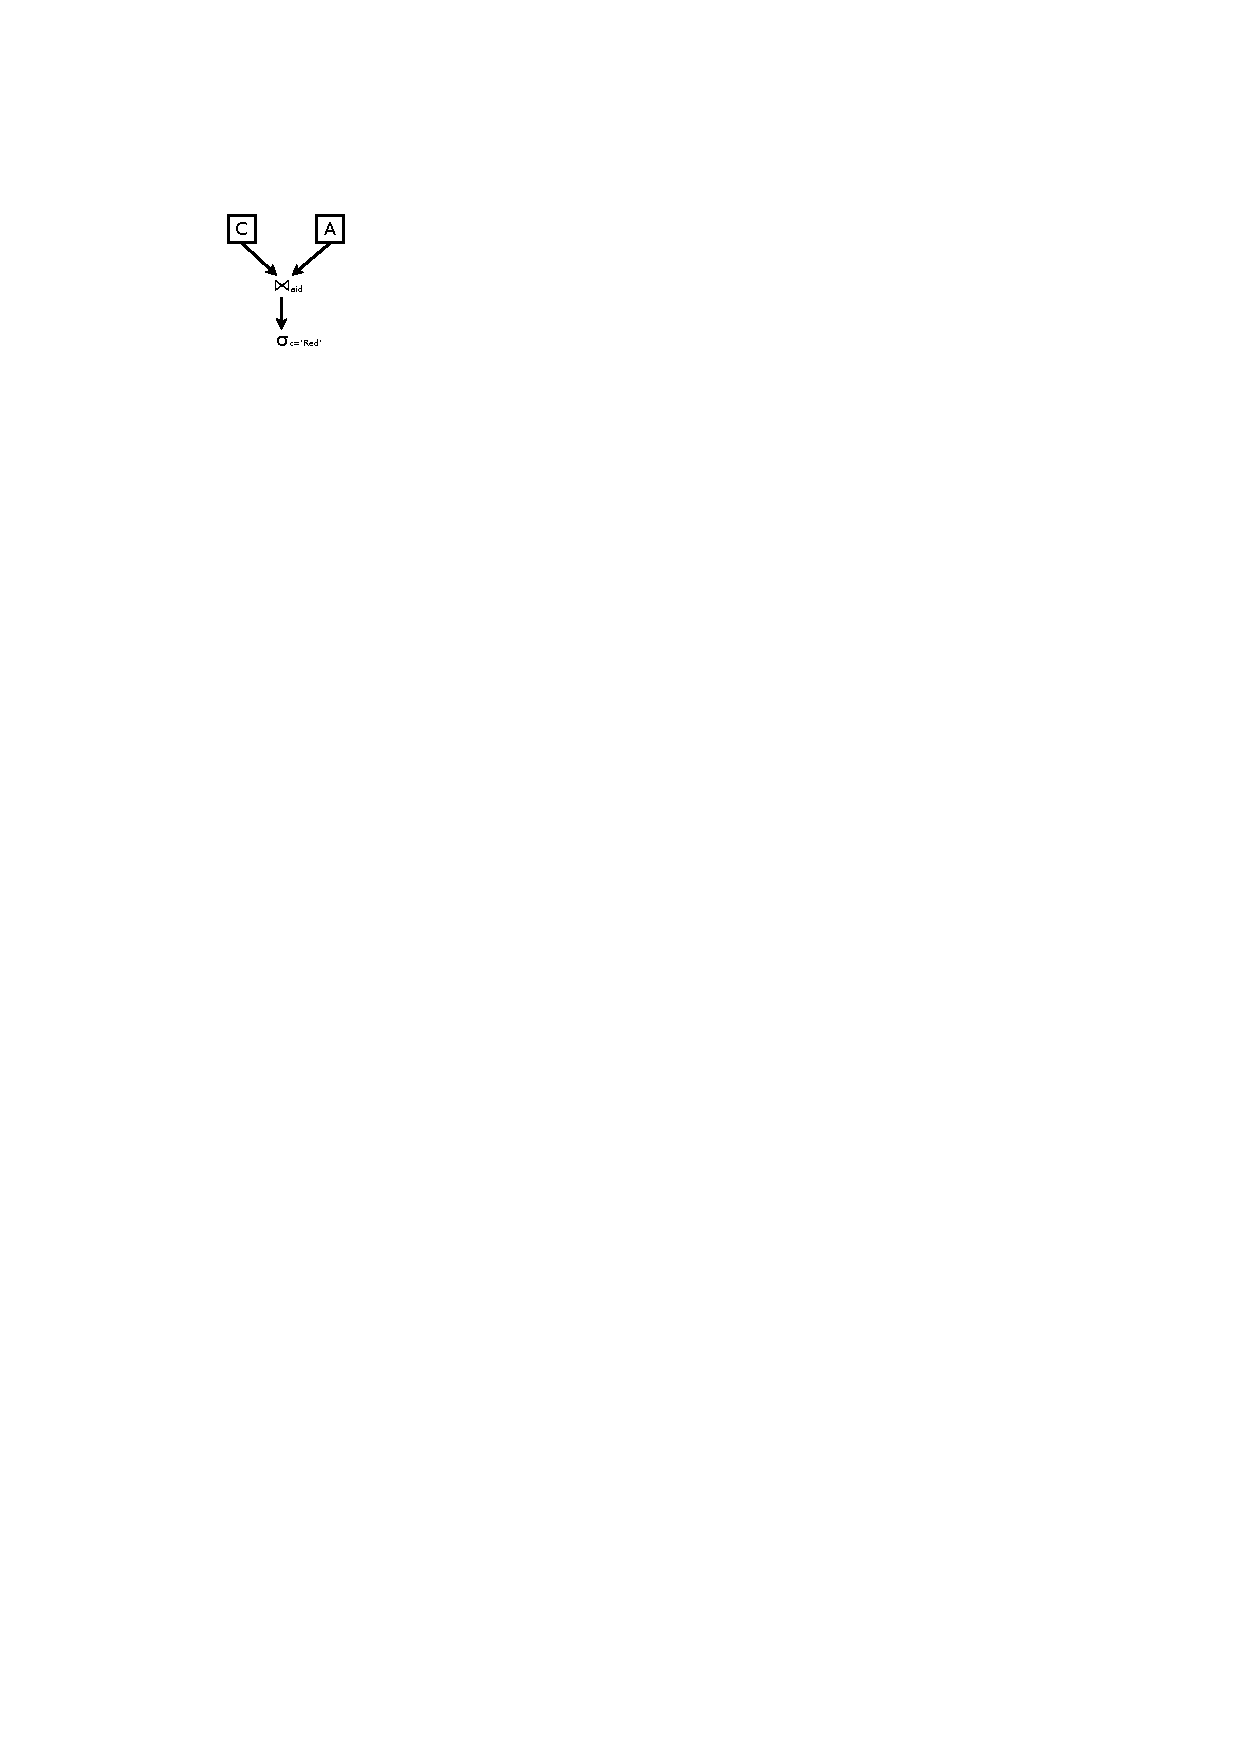
\includegraphics[scale=1.0,trim=3.81cm 23.774cm 15.1cm 3.3cm]{img/relational-algebra}
	\label{fig:query-representations-a}
	\end{minipage}
}
\qquad
\subfloat[toc list entry][Mathematical]{
	\centering
	\begin{minipage}[b]{0.25\linewidth}
	$A = address \\
	C = car \\
	c = color \\
	R = \sigma_{c='Red'}(C\bowtie_{aid} A)$
	\end{minipage}
	\label{fig:query-representations-b}
}
\qquad
\subfloat[toc list entry][SQL]{
	\begin{minipage}[b]{0.35\linewidth}
	\fontfamily{ppl}\ttfamily
	SELECT * \\ FROM
	car, address \\
	WHERE car.aid = address.aid\\AND color = 'Red'
	\end{minipage}
	\label{fig:query-representations-c}
}
\caption{Query representation}
\end{figure}

This chapter describes common database operations, and some more
exotic operations that have recently gained acceptance in the database
community.

\section{Selection and projection}

Selection $\sigma$ is used to select a number of rows from a relation
by specifying a condition. E.g. select every row that has an id below
10. The condition is typically a boolean combination of terms that
have the form $attribute$ op $constant$ or $attribute$ op $attribute$,
where op can be any of the following comparison operators: $<, \leq,
=, \neq, or >$. \cite{dbms}

\begin{lstlisting}[caption={Selection and projection example}]
SELECT id,name
FROM car
WHERE id < 10
\end{lstlisting}

The projection operator $\pi$ is used to extract columns from a
relation, e.g.  select the $id$ of each car. In the process of
optimizing a query it is often reasonable to do projection before
selection to minimize data movement, only the relevant attributes
should be kept. Additionally, projection remove duplicate entries, so
that every row is unique after completion.

\section{Join}

The join operation is one of the most useful operations in relational
algebra and the most common method used to combine information from
two or more relations \cite{dbms}. Join can be defined as the
cross-product of two (or more) relations followed by selection and
projection. However, the cross-product is very big compared to the
join result, so the operator is rarely (never) implemented this way in
practice. Join have received a lot of attention, and there are several
variants of the operation.

Conditional join is most common, this variant accepts a join condition
$c$ and a pair of relation instances as arguments, it returns a
relation instance.

\begin{lstlisting}[caption={Join example}, label={lst:join}]
SELECT * 
FROM car,address
WHERE car.aid = address.id
\end{lstlisting}

Equijoin is a special case of the join operation, where the join
condition consists of only equalities, connected by $\land$. Listing
\ref{lst:join} is an example of equijoin, here the result of a
conditional join would include both car.aid and address.aid, two
identical values, equijoin use projection to remove such redundancies.

Natural join is an additional special case of the join operation where
the equalities are specified on all fields having the same name in
joined relations. The result are guaranteed not to have two fields
with the same name.

\section{Top-$k$}

In many domains, end-users are interested in the most important
(top-$k$) query answers, from a potentially huge solution space.
Answers can be ranked by multiple criteria, like price, location, and
size. Each criterion is weighted, and score is typically calculated as
a weighted sum.

To efficiently produce answers to top-$k$ queries, database management
systems (DBMSs) can use specialized top-$k$ operators like top-$k$ select
and top-$k$ join. An overview of is found in \cite{topksurvey}.

\subsection{Select}

Top-$k$ select is a special case of select, where the $k$ best matches for
a given scoring function is returned. The scoring function is
typically defined as a weighted sum over a set of attributes, i.e.
$f(a,b,c) = 0.5 * a + 0.4 * b + 0.1 * c$. Top-$k$ select requires that
all attributes are contained in one relation.

\begin{minipage}{\textwidth}
\begin{lstlisting}[caption={Top-$k$ select example}, label={lst:topk-select}]
SELECT * 
FROM post
WHERE author='Pete' 
ORDER BY 0.5*comments + 0.4*views + 0.1*likes 
LIMIT 5
\end{lstlisting}
\end{minipage}

The query in listing \ref{lst:topk-select} selects the 5 best posts
authored by Pete, posts are ranked by comments, views, and likes,
respectively.

\subsection{Join}

Top-$k$ join is a generalization of top-$k$ select, where attributes can
be selected from any number of relations. The answer to a top-$k$ join
query is an ordered set of join results according to some provided
function that combines the orders on each input \cite{topkjoin}.
Compared to the normal join operator, top-$k$ can be executed much
faster if a suitable algorithm is used. The algorithm only needs to
return $k$ results and does not necessarily have to join every row in
the relations (as opposed to traditional join).

\begin{lstlisting}[caption={Top-$k$ join example}, label={lst:topk-join}]
SELECT * FROM post,category
WHERE author='Pete' and post.cid = category.cid
ORDER BY 0.5*post.comments + 0.5*category.views
LIMIT 10 
\end{lstlisting}
